\documentclass[11pt,a4paper]{article}
\usepackage[round,authoryear]{natbib} % bibliography style
\bibliographystyle{apalike}

% % --------- packages
\usepackage{latexsym} 
\usepackage{graphicx} 
\frenchspacing 
\usepackage{array}
\usepackage{amsmath}
\usepackage{amssymb}
\usepackage{amsthm}
\usepackage[dvips]{epsfig}
\usepackage{multirow}
\usepackage{booktabs}
\usepackage{rotating, tabularx}
\usepackage{epsf}
\usepackage{psfrag}
\usepackage{pdflscape}
\usepackage{mathrsfs}
\usepackage{bm}
\usepackage[footnotesize,bf]{caption}
% \usepackage[footnotesize]{caption}
\setlength{\captionmargin}{20pt}
\usepackage{caption}
\usepackage{subcaption}
\usepackage{enumerate}
\usepackage{enumitem}
\usepackage{float}
\usepackage{picture}
\usepackage{verbatim}
\usepackage{listings}
\usepackage{color}
\usepackage[dvips,colorlinks,citecolor=black,urlcolor=black,linkcolor=black]{hyperref}
\setlength{\parindent}{0.8cm}  
\setlength{\headsep}{2cm} % by Charlie&Sebastiano to run in non-unix system
% \setlength{\headsep}{1.5cm} % unix system
\lstset{frame=single, language=Matlab, numberstyle=\tiny,
basicstyle=\scriptsize, commentstyle=\tiny}
\usepackage{multirow}
\usepackage{lastpage}
\usepackage[table]{xcolor}% http://ctan.org/pkg/xcolor
\usepackage{setspace}
\usepackage{parskip}


\DeclareMathOperator*{\argmax}{argmax}
\DeclareMathOperator*{\argmin}{argmin}

% define isardSAT colors
% \definecolor{dark_red}{rgb}{0.58, 0.02, 0.02} 
\definecolor{dark_red}{rgb}{0.647, 0.0549, 0.133} 
\definecolor{dark_gray}{rgb}{0.4, 0.4, 0.4} 
\definecolor{light_gray}{rgb}{0.75, 0.75, 0.75} 

\renewcommand{\thefigure}{\arabic{section}-\arabic{figure}}
\renewcommand{\thetable}{\arabic{section}-\arabic{table}}
% \numberwithin{equation}{subsection}
% \renewcommand{\theequation}{equation \arabic{section}-\arabic{table}}
\renewcommand{\theequation}{\arabic{section}-\arabic{equation}}

\renewcommand{\arraystretch}{1.4}
\renewcommand{\contentsname}{Table of contents}
% \pagenumbering{6roman}
\usepackage[titletoc, title, toc, page]{appendix}
\renewcommand{\appendixname}{Annex}
\renewcommand\appendixtocname{Annex}


%%%%%%%%%%%%%%%%%%%%%%%%%%%%%%%%%%%%%%%
\newcommand\projref{JC-DD-ISR-GP-0219}
\newcommand\isdref{ISARD\_ESA\_S6\_P4\_GPP\_ATBD\_1287}
\newcommand\thedate{February 20th, 2024}
\newcommand\issueno{1.b}
\newcommand\activityref{S6 P4 L1 GPP CCN6 }
\newcommand\thetitle{S6 P4 Numerical retracker}
\newcommand\thesubtitle{Algorithms Technical
Baseline Description}
\newcommand\writtenby{Alba Granados and Charlie McKeown}
%%%%%%%%%%%%%%%%%%%%%%%%%%%%%%%%%%%%%%%%


%%% GEOMETRY %%%%%
\usepackage{geometry}
\geometry{a4paper, left=33mm, right=16mm, top=30mm, bottom=45mm}
% \geometry{a4paper, left=33mm, right=16mm, top=30mm, bottom=20mm}

\usepackage{fancyhdr}
%%% DEFINE HEADINGS %%%
\pagestyle{fancy} 
\rhead{\vspace{0.5cm}Project Reference: \projref \\ isardSAT Ref.: \isdref\\ Issue: \issueno / Date: \thedate \\ Page: \thepage\ of \pageref*{LastPage}\vspace{-0.1cm}}
\lhead{$\hspace{-1.5cm}$\raisebox{6mm}{\includegraphics[width=4cm]{fig/logo_isardsat}}}
\cfoot{ }
\lfoot{$\hspace{-1.5cm}$\raisebox{-3mm}{\color{dark_gray}  \textbf{isardSAT}}}
\rfoot{\color{dark_gray}  Numerical retracker -- ATBD}
\renewcommand{\headrule}{\vskip-0\baselineskip \hspace{-1.6cm}\hbox to 1.1\headwidth{\color{light_gray}\leaders\hrule height \headrulewidth\hfill}}
\renewcommand{\headrulewidth}{0.8pt}
\addtolength\headwidth{0cm}
\fancyheadoffset{0.1cm}
% \fancyheadoffset[LE,RO]{\dimexpr\marginparsep+\marginparwidth\relax}



%%% SECTION/SUBSECTION/SUBSUBSECTION headings format - red, font, ... %%%%
\usepackage{titlesec}
\titleformat{\section}
{\Huge\sc \color{dark_red}}% format applied to label+text
{\hspace{-2.5cm}\thesection}% label
{1em}% horizontal separation between label and title body
{}% before the title body
[{\titlerule[0.5pt]}\medskip]% after the title body

\titleformat{\subsection}
{\LARGE\bfseries}
{\hspace{-1.7cm}\thesubsection}
{1.15em}
{}
[]

\titleformat{\subsubsection}
{\large\bfseries}
{\hspace{-1.8cm} \thesubsubsection}
{1.3em}
{}
[]

\setcounter{tocdepth}{4}
\setcounter{secnumdepth}{4}
\titleformat{\paragraph}
{\normalsize\bfseries}
{\hspace{-1.8cm} \theparagraph}
{0.8em}
{}
% \titlespacing*{\paragraph}
% {0pt}{3.25ex plus 5ex minus .2ex}{1.5ex plus .2ex}



%%% appendix pagestyle ... %%%%
\fancypagestyle{simple}{%
    \fancyhead{}
    \lhead{$\hspace{-1.5cm}$\raisebox{-13mm}{\includegraphics[width=4cm]{fig/logo_isardsat}}}
    \renewcommand{\headrulewidth}{0pt}
    \renewcommand{\footrulewidth}{0.4pt}% default is 0pt
    \renewcommand{\footrule}{\hbox to\headwidth{\color{light_gray}\leaders\hrule height \footrulewidth\hfill}}
    \rfoot{}
    \lfoot{}

}

%%% cover pagestyle ... %%%%
\fancypagestyle{cover}{%
    \fancyhead{}
    \lhead{$\hspace{-1.5cm}$\raisebox{-13mm}{\includegraphics[width=4cm]{fig/logo_isardsat}}}
    \renewcommand{\headrulewidth}{0pt}
    \renewcommand{\footrulewidth}{0pt}% default is 0pt
    \renewcommand{\footrule}{\hbox to\headwidth{\color{light_gray}\leaders\hrule height \footrulewidth\hfill}}
    \rfoot{}
    \lfoot{}
}

% % Running line numbers:
% \linenumbers
% \setlength\linenumbersep{15pt}
% \renewcommand\linenumberfont{\normalfont\tiny\sffamily\color{red}}




%%%%%%%%%%%%%%%%%%%%%%%%%%%%%%%%%%%%%%%%%%%%%%%%%%%%%%%%%%%%%%%%
%%%%% -------------------- DOCUMENT ------------------- %%%%%%%%
%%%%%%%%%%%%%%%%%%%%%%%%%%%%%%%%%%%%%%%%%%%%%%%%%%%%%%%%%%%%%%%%


\begin{document}

\setlength{\parskip}{8pt}

%%%%%%%%%%%%%%% TITLE PAGE %%%%%%%%%%%%%%%%%%%%%%%%%%%%%%
%%%%%%%%%%%%%%%%%%%%%%%%%%%%%%%%%%%%%%%%%%%%%%%%%%%%%%%%%%
% 

\thispagestyle{cover}

% \begin{titlepage}

% \vspace*{-1.75cm}
% \includegraphics[width=4cm]{fig/logo_isardsat.png}
        
    \begin{center}
        \vspace*{3.5cm}
                
        \begin{flushright}
        
        \begin{spacing}{2.5}        
        {\Huge \textbf{\thetitle}}
        
        \vspace{2cm}
        {\Huge \textbf{-- \thesubtitle $\;$--}}
        \end{spacing}

        \end{flushright}
            
        \vspace{7.5cm}
        \begin{flushright}
        \large
        Project Reference:  \projref\\ 
        isardSAT Reference: \isdref \\
        Issue: \issueno \\
        
        \bigskip
        Prepared by: \writtenby\\
%         Reviewed by: \\
%         Approved by:\\
        \thedate \\
        Activity: \activityref
        \end{flushright}
    
    \end{center}
% \end{titlepage}




%%%%%%%%%%%%%%%%%%%%%%% BLANK PAGE %%%%%%%%%%%%%%%%%%%%%
%%%%%%%%%%%%%%%%%%%%%%%%%%%%%%%%%%%%%%%%%%%%%%%%%%%%%%%%
\clearpage
\newpage

\begin{center}
$\quad$

\vspace{0.4\textheight}

This page has been intentionally left blank

\end{center}



%%%%%%%%%%%%%%%%%%%%%%%%%%%%%%%%% PREAMBLE %%%%%%%%%%%%%%%%%%
%%%%%%%%%%%%%%%%%%%%%%%%%%%%%%%%%%%%%%%%%%%%%%%%%%%%%%%%%%%%
\clearpage
\newpage


\titleformat{\section} % section title in black and bfseries
{\huge\bfseries}
{ \thesection}
{1em}
{}
[]
%%%%%%%%%%%%%%%%%%%%%%%%%%%%%%%%%%%%
\section*{ Change Record}
\addcontentsline{toc}{section}{\protect\numberline{}\hspace{-0.4cm}Change Record}%

\begin{table}[ht!]
     \centering 
\begin{tabular}{|m{0.25\textwidth}|m{0.15\textwidth}|m{0.15\textwidth}|m{0.325\textwidth}|}
  \hline
  \cellcolor{dark_red} \color{white}{\bf Date} & \cellcolor{dark_red} \color{white}{\bf Issue} & \cellcolor{dark_red} \color{white}{\bf Section} & \cellcolor{dark_red} \color{white}{\bf Comment} \\
  \hline
  September 22nd, 2023 & 1.a & all & First issue\\
  \hline
    February 20th, 2024 & 1.b & \S\ref{sec:input_var_aux_data_selection}, \S\ref{sec:output_var_aux_data_selection}, \S\ref{sec:input_var_pre_processing}, \S\ref{sec:output_var_pre_processing} & Include Input/Output variable lists\\
  \hline
\end{tabular}
\end{table}


%%%%%%%%%%%%%%%%%%%%%%%%%%%%%%%%%%%%%
\section*{Control Document}
\addcontentsline{toc}{section}{\protect\numberline{}\hspace{-0.4cm}Control Document}%

\begin{table}[ht!]
     \centering 
\begin{tabular}{|m{0.18\textwidth}|m{0.47\textwidth}|m{0.25\textwidth}|}
  \hline
  \cellcolor{dark_red} \color{white}{\bf Process} & \cellcolor{dark_red} \color{white}{\bf Name} & \cellcolor{dark_red} \color{white}{\bf Date} \\
  \hline
  Written by: & \writtenby & \thedate\\
  \hline
  Reviewed by: &  Ester Vendrell & \thedate \\
  & M\`onica Roca i Aparici &\\
  \hline
  Approved by: & -- & \thedate\\
  \hline
\end{tabular}
\end{table}

%%%%%%%%%%%%%%%%%%%%%%%%%%%%%%%%%%%%
\section*{Distribution List}
\addcontentsline{toc}{section}{\protect\numberline{}\hspace{-0.4cm}Distribution List}%

\begin{table}[ht!]
     \centering 
\begin{tabular}{|m{0.46\textwidth}|m{0.47\textwidth}|}
  \hline
  \cellcolor{dark_red} \color{white}{\bf Company } & \cellcolor{dark_red} \color{white}{\bf Name} \\
  \hline
    ESA & Marco Fornari \\
        & Luisella Giulicchi \\
     & Robert Cullen \\
    \hline
    isardSAT & Ester Vendrell \\
    & M\`onica Roca i Aparici \\

    \hline
\end{tabular}
\end{table}


%%%%%%%%%%%%%%%%%%%%%%%% TABLE OF CONTENTS %%%%%%%%%%%%%
%%%%%%%%%%%%%%%%%%%%%%%%%%%%%%%%%%%%%%%%%%%%%%%%%%%%%%%
\clearpage
\newpage

\begin{footnotesize}
\tableofcontents
\end{footnotesize}

%%%%%%%%%%%%%%%%% LIST OF FIGURES NOMENCLATURE ETC. %%%%%
\clearpage
\newpage
% \section*{List of Figures}
\addcontentsline{toc}{section}{\protect\numberline{}\hspace{-0.4cm}List of Figures}%

\listoffigures


%%%%%%%%%%%%%%%%
\clearpage
\newpage
\addcontentsline{toc}{section}{\protect\numberline{}\hspace{-0.4cm}List of Tables}%

\listoftables


%%%%%%%%%%%%%%%%%%%%%%%%%%%%%%%%%%%%%%%
\clearpage
\newpage
\section*{List of Symbols}
\addcontentsline{toc}{section}{\protect\numberline{}\hspace{-0.4cm}List of Symbols}%

\paragraph*{Indexes:}
\begin{table}[H]
\hspace{-0.2cm}\begin{tabular}{m{0.15\textwidth}m{0.8\textwidth}}

$i$  & Beam number \\

$l_i$ & Beam index \\

$j$ & Two-way incremental time index \\

$t_j$ & Two-way incremental time \\

$t_j^\prime$ & Two-way incremental time after delay compensation \\

$b^\prime_i$ & Index of the beam pointing to a specific surface \\

\end{tabular}
\end{table}


\paragraph*{Variables, constants and functions:}
\begin{table}[ht!]
\hspace{-0.2cm}\begin{tabular}{m{0.15\textwidth}m{0.8\textwidth}}

$\alpha$ & Earth curvature \\

$c$ & Light Velocity \\

$\delta\theta_{look}$ & Angular Doppler resolution \\

$\delta t_{l_i}$ & Time delay applied to beam $l_i$ \\

$e_{meas}$ & Noise floor of the measured multilooked power waveform \\

$e_{model}$ & Noise floor of the modelled multilooked waveform \\

$G_0$ & Boresight antenna gain \\

$\gamma$ & Beamwidth parameter \\

$\text{H}_\text{mask}(t_j^\prime, l_i)$ & delay/Doppler mask matrix \\

$H_s$ & Significant wave height \\

$j_0$ & First range gate considered in the fitting \\

$j_L$ & Leading edge sample \\

$j_N$ & Range gate before leading edge with notable power increase \\

$j_P$ & Range gate closest to leading edge with a power peak \\

$k_0$ & Epoch \\

$\theta_p$, $\alpha_r$ & Mispointing angles \\ 

$\bm{\theta}$ & Three-dimensional parameter vector \\

$\theta_{3dB}$ & Half-power antenna beamwidth \\




\end{tabular}
\end{table}


\begin{table}[ht!]
\hspace{-0.2cm}\begin{tabular}{m{0.15\textwidth}m{0.8\textwidth}}

$\theta_{look}$ & Look angles \\

$\bm{\theta}_0$ & Initial guess of the geophysical parameters estimates vector \\

$\theta_{look, b_i^\prime}$ & Look angle of the $i$-th beam pointing to a specific surface \\

$\lambda_s$ & Ocean skewness \\

$\lambda$ & Radar wavelength\\

$h$ & Satellite altitude \\


$N_s$ & Number of range samples (non zero-padded)\\

$N_p$ & Number of pulses per burst  \\

$N_{eff}$ & Number of effective looks \\   


$OS\_AL$ & Oversampling along track \\

$OS\_AC$ & Oversampling across track \\


$P_u$ & Waveform amplitude \\

$P(t_j, l_i)$ & Power waveform at time $t_j$ and Doppler index $l_i$ \\

$p(t_j)$ & Probability density function of the heights at time $t_j$ \\

$\text{P}_\text{FSIR}(t_j, l_i)$ & Flat surface impulse response at time $t_j$ and Doppler index $l_i$\\

$\text{P}_\text{I}(t_j, l_i)$ & Average surface impulse response at time $t_j$ and Doppler index $l_i$\\

$\text{P}_\text{PTR}(t_j, l_i)$ & Point target response at time $t_j$ and Doppler index $l_i$ \\

$\text{P}_\text{DC}^\text{mask}(t_j, l_i)$ & Power waveform after delay compensation and masking \\

$\text{P}_\text{AIR}(l_i)$ & Azimuth point target response \\

$\text{P}_\text{RIR}(t_j)$ & Range point target response \\

$\text{P}_\text{DC}(t_j^\prime, l_i)$ & Waveforms forming the stack after delay compensation \\

PRF & Pulse repetition frequency\\

PRI & Pulse repetition interval\\

$R$ & Earth's radius \\

$r_j$ & Residual of the optimisation function \\ 

$\rho(t_j)$ & Range projected on the surface \\

$\rho_L(\cdot)$ & Loss function \\

$s_j \equiv s(t^\prime_j)$ & Noise-free modelled multilooked waveform \\

$\tilde{s}(t^\prime_j)$ & Noisy modelled multilooked waveform \\

$\sigma_s$ & Root mean square height relative to the mean sea level \\

$\sigma^0$ & Normalized backscatter radar cross section \\ 

\end{tabular}
\end{table}

\newpage
\clearpage

.
\vspace{-2cm}
\begin{table}[ht!]
\hspace{-0.2cm}\begin{tabular}{m{0.15\textwidth}m{0.8\textwidth}}


$t$ & Two-way incremental time \\

$T_s$ & Sampling period \\

$U(\cdot)$ & Heaviside function \\

$\bm{v}_s$ & Satellite velocity vector \\

$y_{t_j, l_i}$ & Along track distance at time $t_j$ and Doppler look $l_i$ \\

$ZP$ & Zero padding factor \\

$\phi_{t_j, l_i}$ & Azimuth angle at time $t_j$ and Doppler index $l_i$ \\

$\psi_j$ & Measured power waveform at sample $j$ \\

$\psi_{max}$ & Maximum power of the measured power waveform\\

\end{tabular}
\end{table}


% \begin{table}[htb!]
% \hspace{-0.2cm}\begin{tabular}{m{0.15\textwidth}m{0.8\textwidth}}
% \multicolumn{2}{l}{\bf Mathematical operations:} \\
% 
% $E[\cdot]$ & Expectation\\
% 
% \end{tabular}
% \end{table}


% %%%%%%%%%%%%%%%%%%%%%%%%%%%%%%%%%%%%%%%
% \clearpage
% \newpage
% \section*{List of Functions}
% \addcontentsline{toc}{section}{\protect\numberline{}\hspace{-0.4cm}List of Functions}%
% 
% 
% \begin{table}[htb!]
% \hspace{-0.2cm}\begin{tabular}{m{0.15\textwidth}m{0.8\textwidth}}
% 
% $x(0)$ & First component of vector $x$\\
% 
% \end{tabular}
% \end{table}



% %%%%%%%%%%%%%%%%%%%%%%%%%%%%%%%%%%%%%%%
% \clearpage
% \newpage
% \section*{Nomenclature}\label{sec:nomenclature}
% \addcontentsline{toc}{section}{\protect\numberline{}\hspace{-0.4cm}Nomenclature}%
% 
% 
% \noindent{\bf Latin letters:}
% \begin{table}[htb!]
% \hspace{-0.2cm}\begin{tabular}{m{0.1\textwidth}m{0.9\textwidth}}
% $A$ & Area illuminated by the radar beam \\
% 
% \end{tabular}
% \end{table}
% 
% \noindent{\bf Greek letters:}
% \begin{table}[ht!]
% \hspace{-0.2cm}\begin{tabular}{m{0.1\textwidth}m{0.9\textwidth}}
% $\bm{\Gamma}_e$ & Noise covariance matrix \\ % Alba: this may change when we merge well Noise section and MAP
% 
% $\xi$ & Residual norm \\
% 
% \end{tabular}
% \end{table}



%%%%%%%%%%%%%%%%%%%%%%%%%%%%%%%%%%%%%%%%%%%%%%%%%%%%%%%%%
%%%%%%%%%%%%%%%%%%%% BEGIN ACTUAL DOCUMENT %%%%%%%%%%%%%%%
%%%%%%%%%%%%%%%%%%%%%%%%%%%%%%%%%%%%%%%%%%%%%%%%%%%%%%%%%
\clearpage
\newpage

% \pagenumbering{arabic} % start arabic paging
% \setcounter{page}{5}

\titleformat{\section} % back to section heading format
{\Huge\sc \color{dark_red}}
{\hspace{-2.1cm} \thesection}
{1.1cm}
{}
[\vspace{-0.7\baselineskip}\hspace{-1.7cm}{\titlerule[0.5pt]}\medskip]


%%%%%%%%%%%%%%%%%%%%%%%%%%%%%%%%%%%%%%%%%%%%%%%%%%%%%%%
\section{Introduction}\label{sec:introduction}

\subsection{Scope of the document}

This document contains the theoretical description and implementation of a numerical retracker performed as part of the  WP160 of the CCN \#6 [AD. 2] of the contract Poseidon-4 Ground Processor Prototype [AD. 3].

The scope of this document is to describe the algorithms technical baseline of the retracker for Poseidon-4 (P4), the Sentinel-6 (S6) mission altimeter.


% \subsection{Document organization}
% 
% This document is organised with the following main sections: \S\ref{sec:introduction} provides the scope of this deliverable, the reference list and a brief description of the deliverable's structure; \S\ref{sec:descrition_ascat} introduces 


\subsection{Acronyms}

\begin{table}[ht!]
\hspace{-0.2cm}\begin{tabular}{m{0.15\textwidth}m{0.8\textwidth}}

AIR & Azimuth impulse response \\

CAL1 & Calibration file \\

DDP & delay/Doppler Processing (usually written as SAR processing) \\


EUMETSAT & European Organisation for the Exploitation of Meteorological Satellites \\


ESA & European Space Agency  \\

FFT & Fast Fourier Transform \\

GMSL & Global mean sea level \\

HR & High Resolution (referred to the DDP products) \\


L1B & Level-1B. Output file with fully calibrated multilooked unfocussed SAR power echoes for HR \\


LSQ & Least-squares \\

LUT & Look-up-table \\

MSE & Mean square error \\

P4 & Poseidon-4 \\

PDAP & Payload Data Acquisition and Processing \\


PRI & Pulse Repetition Interval \\

PTR & Point Target Response \\

PRF & Pulse Repetition Frequency \\

RIR & Range Impulse Response  \\



\end{tabular}
\end{table}

\begin{table}[ht!]
\hspace{-0.2cm}\begin{tabular}{m{0.15\textwidth}m{0.8\textwidth}}
RMS & Root-mean-square \\

SSH & Sea surface height \\

S6 & Sentinel-6 \\

SAR & Synthetic Aperture Radar \\

UTC & Universal Time Coordinated \\

ZP &  Zero Padding \\ 



\end{tabular}
\end{table}



\subsection{Reference}

Unless stated otherwise, the latest issue of the documents at the date of the issue of this document is valid. The valid issue of the documents is recorded in the document status list. In the following, each document item consists of 3 entries: bookmark ID (specific to this document), document title.


\subsubsection{Applicable documents}

\begin{itemize}
 \item [AD. 1] Sentinel-6 P4 L1 GPP - Algorithm Technical Baseline Description. JC-DS-ISR-SY-0013, issue 7.a, 6 November 2019.
 \item [AD. 2] Contract Change Notice No. 6 to Contract No. 4000112536/14/NL/BJ

\end{itemize}


\subsubsection{Reference documents}

\begingroup 
\renewcommand{\section}[2]{}%
\bibliography{library.bib} % uncomment: path to .bib

\endgroup


\subsection{Assumptions}


In the following sub-section we provide a list of further assumptions used in the development of this software.

\subsubsection{L1B input products}

The L1B input files used by the retracker are listed and defined in \S\ref{sec:l1b_products}.

\subsubsection{Auxiliary files}

The software configuration and constant files shall be managed by the user. The instrument characterisation file shall be defined by the instrument team. The list of auxiliary files used by the software is provided in \S\ref{sec:auxiliary_files}



\subsection{Conventions and remarks}

\subsubsection{Scope of sections}

Each of the algorithms described in this document follows the same general structure. The purpose and scope section gives a brief description of the algorithm, followed by a data block diagram that shows the main steps that are performed. The mathematical description included in each algorithm provides a description of the algorithm in mathematical terms. The terminology used in the mathematical description is usually generic and uses mathematical symbols. After that, the input and output variables destination is provided in order to ease the understanding of the whole chain.


\subsubsection{Block diagrams legend}

All the block diagrams have the same legend, for the sake of clarity. The legend is shown in Figure~\ref{fig:legend_blockdiagram}.

\begin{figure}[htb!]\centering
  \centering
  
\includegraphics[width=0.2\textwidth]{fig/legend_blockdiagram}
  \caption[ Colour and symbols diagram legend]{Colour and symbols diagram legend.}
  \label{fig:legend_blockdiagram}
\end{figure}


\subsubsection{Product types}

The different product types according to their level of processing are:

\begin{itemize}
 \item L1B HR: Fully calibrated and geolocated power echoes.
 \item CAL1 L1B Pulse CAL, CAL1 L1B SAR: output of calibration processor
 \item L2 HR: output ocean geophysical retrievals not corrected for atmospheric and geophysical effects.

\end{itemize}




\clearpage
\newpage
%%%%%%%%%%%%%%%%%%%%%%%%%%%%%%%%%%%%%%%%
\section{Input files description}\label{sec:inputfiles_description}

This section contains the description and reference of all the input data files. These files can be divided
in:

\begin{itemize}
 \item L1B products
 \item Calibration products
 \item Auxiliary files
\end{itemize}

The following chapters provide a list of the input files with a brief description, and Table~\ref{tab:input_data} below indicates for each input file if it is mandatory or optional.

\begin{table}[ht!]
     \centering 
     \caption[Input data list of the retracker]{Input data list of the retracker}\label{tab:input_data}
\begin{tabular}{|m{0.3\textwidth}|m{0.15\textwidth}|}
\hline
  \multicolumn{1}{c}{\cellcolor{dark_red} \color{white}\textbf{Data}} & \multicolumn{1}{c}{\cellcolor{dark_red} \color{white}\textbf{}} \\
  \hline
  L1B HR & Mandatory \\
CAL1 L1B Pulse CAL & Optional \\
  CAL1 L1B SAR & Optional \\
  Characterisation file & Mandatory \\
  Retracker configuration file & Mandatory \\
  Constant file & Mandatory \\
  \hline
\end{tabular}
\end{table}



\subsection{L1B products}\label{sec:l1b_products}


\subsubsection{L1B HR product}

The L1B HR product is the final output of the L1 HR processor. It contains geo-located and fully calibrated multilooked High Resolution power echoes in Ku-band.


\subsection{Calibration products}\label{sec:l1bcal_products}

\subsubsection{CAL1 L1B Pulse CAL product}

The CAL1 L1B Pulse CAL is the output of the Pulse CAL Processor. It contains oversampled CAL1 power waveforms along the orbit for Ku-band.
 
\subsubsection{CAL1 L1B SAR product}

The CAL1 L1B SAR is the output of the CAL1 SAR Processor. It contains an oversampled CAL1 power waveforms for Ku-band. 


\subsection{Auxiliary files}\label{sec:auxiliary_files}


\subsubsection{Characterisation file (CHD)}\label{sec:chd}

The characterisation file contains the system on-ground characterisation. 

\subsubsection{Retracker Configuration file (CNF)}\label{sec:cnf}

The configuration file contains all processing parameters, which can be modified by the user.

\subsubsection{Constants file (CST)}\label{sec:cst}

The constants file contains the main physical constants used by the processor.




\clearpage
\newpage
%%%%%%%%%%%%%%%%%%%%%%%%%%%%%%%%%%%%%%
\section{Auxiliary data selection}

This section describes the procedures to select the right set of the parameters of the different calibration files.

\subsection{CAL1 L1B selection}

\subsubsection{Purpose and scope}

The purpose of this algorithm is to select the impulse response stored in CAL1 L1B products according to the processing flags defined in the retracker configuration file.

\subsubsection{Data block diagram}


\begin{figure}[htb!]\centering
  \centering
  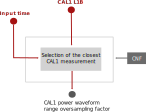
\includegraphics[width=0.45\textwidth]{fig/cal1_data_selection}
  \caption[CAL1 Pulse CAL selection block diagram]{CAL1 Pulse CAL selection block diagram. CAL1 SAR products contain a sole measurement.}
  \label{fig:cal1_selection_diagram}
\end{figure}


\subsubsection{Mathematical description}

The processor will check the \url{PTR_type_ac} retracker configuration flag to select the type of impulse response in range (RIR). If it is set to \texttt{'numerical'}, then follow the next steps.

The source is defined by the user in the \texttt{run\_} file. The processor will check whether this source corresponds to a CAL1 L1B Pulse CAL or a CAL1 L1B SAR product. If a Pulse CAL file is detected, then for each altimeter time tag (in UTC), the selected values corresponds to the closest CAL1 time tag (in UTC) from the L1B Pulse Cal processing product. Alternatively, a sole measurement is stored in the CAL1 product, and this is the one selected.


\subsubsection{Input variable list}\label{sec:input_var_aux_data_selection}


\begin{table}[ht!]
     \centering 
     \caption[Input variable list of the Auxiliary data selection]{Input variable list of the Auxiliary data selection}\label{tab:input_var_aux_data_selection}
\begin{tabular}{|m{0.3\textwidth}|m{0.45\textwidth}|m{0.08\textwidth}|m{0.08\textwidth}|}
  \hline
  \centering \cellcolor{dark_red} \color{white}{\bf Field name} & \centering \cellcolor{dark_red} \color{white}{\bf Description} & \cellcolor{dark_red} \color{white}{\bf Units} & \cellcolor{dark_red} \color{white}{\bf Type}\\
  \hline
  time\_l1b & Time in UTC of the L1B HR product & s & double \\
  \hline
  time\_l1CAL & Time in UTC of the CAL1 L1B product & s & double \\
  \hline
  PTR\_type\_ac & String indicating the PTR across track used for the convolutional model: 'analytical' (sinc), 'numerical' & -- & string \\

    \hline
  
\end{tabular}
\end{table}

\subsubsection{Output variable list}\label{sec:output_var_aux_data_selection}

\begin{table}[ht!]
     \centering 
     \caption[Output variable list of the Auxiliary data selection]{Output variable list of the Auxiliary data selection}\label{tab:output_var_aux_data_selection}
\begin{tabular}{|m{0.3\textwidth}|m{0.45\textwidth}|m{0.08\textwidth}|m{0.08\textwidth}|}
  \hline
  \centering \cellcolor{dark_red} \color{white}{\bf Field name} & \centering \cellcolor{dark_red} \color{white}{\bf Description} & \cellcolor{dark_red} \color{white}{\bf Units} & \cellcolor{dark_red} \color{white}{\bf Type}\\
  \hline
  index\_from\_l1CAL & Array of indices of the CAL1 time vector closest to the L1B HR time vector & -- & int \\
    \hline
  cal1\_power\_waveform & The CAL1 waveform corresponding to the current index\_from\_l1CAL index, converted to Watt via waveform\_scale\_factor & W & double\\
  \hline
  range\_oversampling\_factor & Oversampling factor applied to the CAL1 waveform & -- & int \\
    \hline
\end{tabular}
\end{table}

\clearpage
\newpage
%%%%%%%%%%%%%%%%%%%%%%%%%%%%%%%%%%%%%%
\section{Numerical retracker}\label{sec:retracker}


\subsection{Introduction}\label{sec:retracker_intro}

Cite like this \citep{Ray2015a} or \citep{Ray2015a,Nelder1965}

\subsection{Pre-processing}\label{sec:pre-processing}

\subsubsection{Purpose and scope}

The objective of this processing step is to generate...

\subsubsection{Block diagram}

The block diagram depicted in Figure~\ref{fig:L2_preprocessing_blockdiagram} illustrates the main pre-processing steps.

\begin{figure}[htb!]\centering
  \centering
  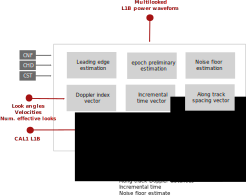
\includegraphics[width=0.7\textwidth]{fig/L2_preprocessing_blockdiagram}
  \caption[Pre-processing block diagram]{Pre-processing block diagram.}
  \label{fig:L2_preprocessing_blockdiagram}
\end{figure}


\subsubsection{Mathematical description}

\paragraph{Leading edge estimation}\label{sec:leading_edge}

An estimate of the leading edge... 

\paragraph{Incremental time}\label{sec:preprocessing_time_incr}

The two-way incremental ranging time vector $t$, dependent on the epoch $k_0$, is equally spaced and ranges from 
\begin{subequations}
\begin{equation}
t_0=\biggl(-\Bigl(N_s-\frac{N_s}{2}\Bigr)\texttt{ZP}+\Bigl(\frac{Ns\cdot\texttt{ZP}}{2}-k_0\Bigr)\biggr)\cdot \frac{T_s}{\texttt{ZP}}
\end{equation}
to 
\begin{equation}
t_{N_s\cdot\texttt{ZP}\cdot\texttt{OS\_AL}-1}=\biggl(\Bigl(N_s-\frac{N_s}{2}\Bigr)\texttt{ZP}+\Bigl(\frac{Ns\cdot\texttt{ZP}}{2}-k_0\Bigr)\biggr)\cdot \frac{T_s}{\texttt{ZP}}
\end{equation}
\end{subequations}
where ...






\subsubsection{Input variable list}\label{sec:input_var_pre_processing}



\subsubsection{Output variable list}\label{sec:output_var_pre_processing}





\clearpage
\newpage
%%%%%%%%%%%%%%%%%%%%%%%%%%%%%%%%%%%%%%%%%%%%%%%%%%%%%%%
\appendix
\setcounter{equation}{0}
\renewcommand{\theequation}{\thesection-\arabic{equation}}
\renewcommand{\thefigure}{\thesection-\arabic{figure}}
\renewcommand{\thetable}{\thesection-\arabic{table}}

\titleformat{\section} % back to section heading format with word Annex
{\Huge\sc \color{dark_red}}
{\hspace{-2.1cm} \appendixname\hspace{0.3cm}\thesection.}
{1.1cm}
{}
[\vspace{-0.7\baselineskip}\hspace{-1.7cm}{\titlerule[0.5pt]}\medskip]

\thispagestyle{simple} % first page of appendix = same style front cover

\addcontentsline{toc}{section}{\appendixname}
\section{Flat surface impulse response with non-zero mispointing}\label{annex:annex1}


\subsection{Purpose and scope}

\subsection{Mathematical description}




% \clearpage
% \newpage
% %%%%%%%%%%%%%%%%%%%%%%%%%%%%%%%%%%%%%%%%%%%%%%%%%%%%%%%
% \section{Title Annex}\label{annex:annex2}




%%%%%%%%%%%%%%%%%%%%%%%%% BLANK PAGE END OF DOC. %%%%%
%%%%%%%%%%%%%%%%%%%%%%%%%%%%%%%%%%%%%%%%%%%%%%%%%%%%%%
\clearpage
\newpage

\pagestyle{fancy}

\centering
$\quad$

\vspace{0.4\textheight}

End of document



    
\end{document}




%%%%%%%%%%%%%%%%%%%%%%%%%%%%%%%%%%%%%%%%%%%%%%%%%%%%%%%%%%%%%%%%
%%%%% -------------------- figure, tables, etc. ------------------- %%%%%%%%
%%%%%%%%%%%%%%%%%%%%%%%%%%%%%%%%%%%%%%%%%%%%%%%%%%%%%%%%%%%%%%%%


% \begin{figure}[htb!]\centering
%   \centering
%   \includegraphics[width=0.9\textwidth]{}
%   \caption[ ]{}
%   \label{}
% \end{figure}
% 
% \begin{figure}[htb!]\centering   
%   \subfloat[]{\label{}\includegraphics[width=0.4\textwidth]{}}$\;$
%   \subfloat[]{\label{}\includegraphics[width=0.4\textwidth]{}}
%   \caption[ ]{}
%   \label{}
% \end{figure}
% 
% \begin{table}[h!]
% \centering
% \begin{tabular}{ c|c } \hline\hline
% 
% \end{tabular}
% \caption{ }
% \label{ }
% \end{table}
